\begin{itemize}
\item Definition: Semantic segmentation means assigning a class label to each of the computed segments example: Road, traffic lights, lanes. Examples: Fully CNN(2015), SegNet(2015), ENet(2016), LinkNet(2017). 
\item Semantic Segmentation is used to detect road in the absence of clear road-lane separation
\item Present developments in Semantic Segmentation on autonomous vehicles
   \subitem SqueezeNet(2016) was able to demonstrate the increase in accuracy of AlexNet using 50 times less parameteres by tweaking with the architectures
   \subitem ENet(2016) could replicate the Semantic Segmentation on real time
\end{itemize}
  \begin{minipage}{0.16\textwidth}
\centering
  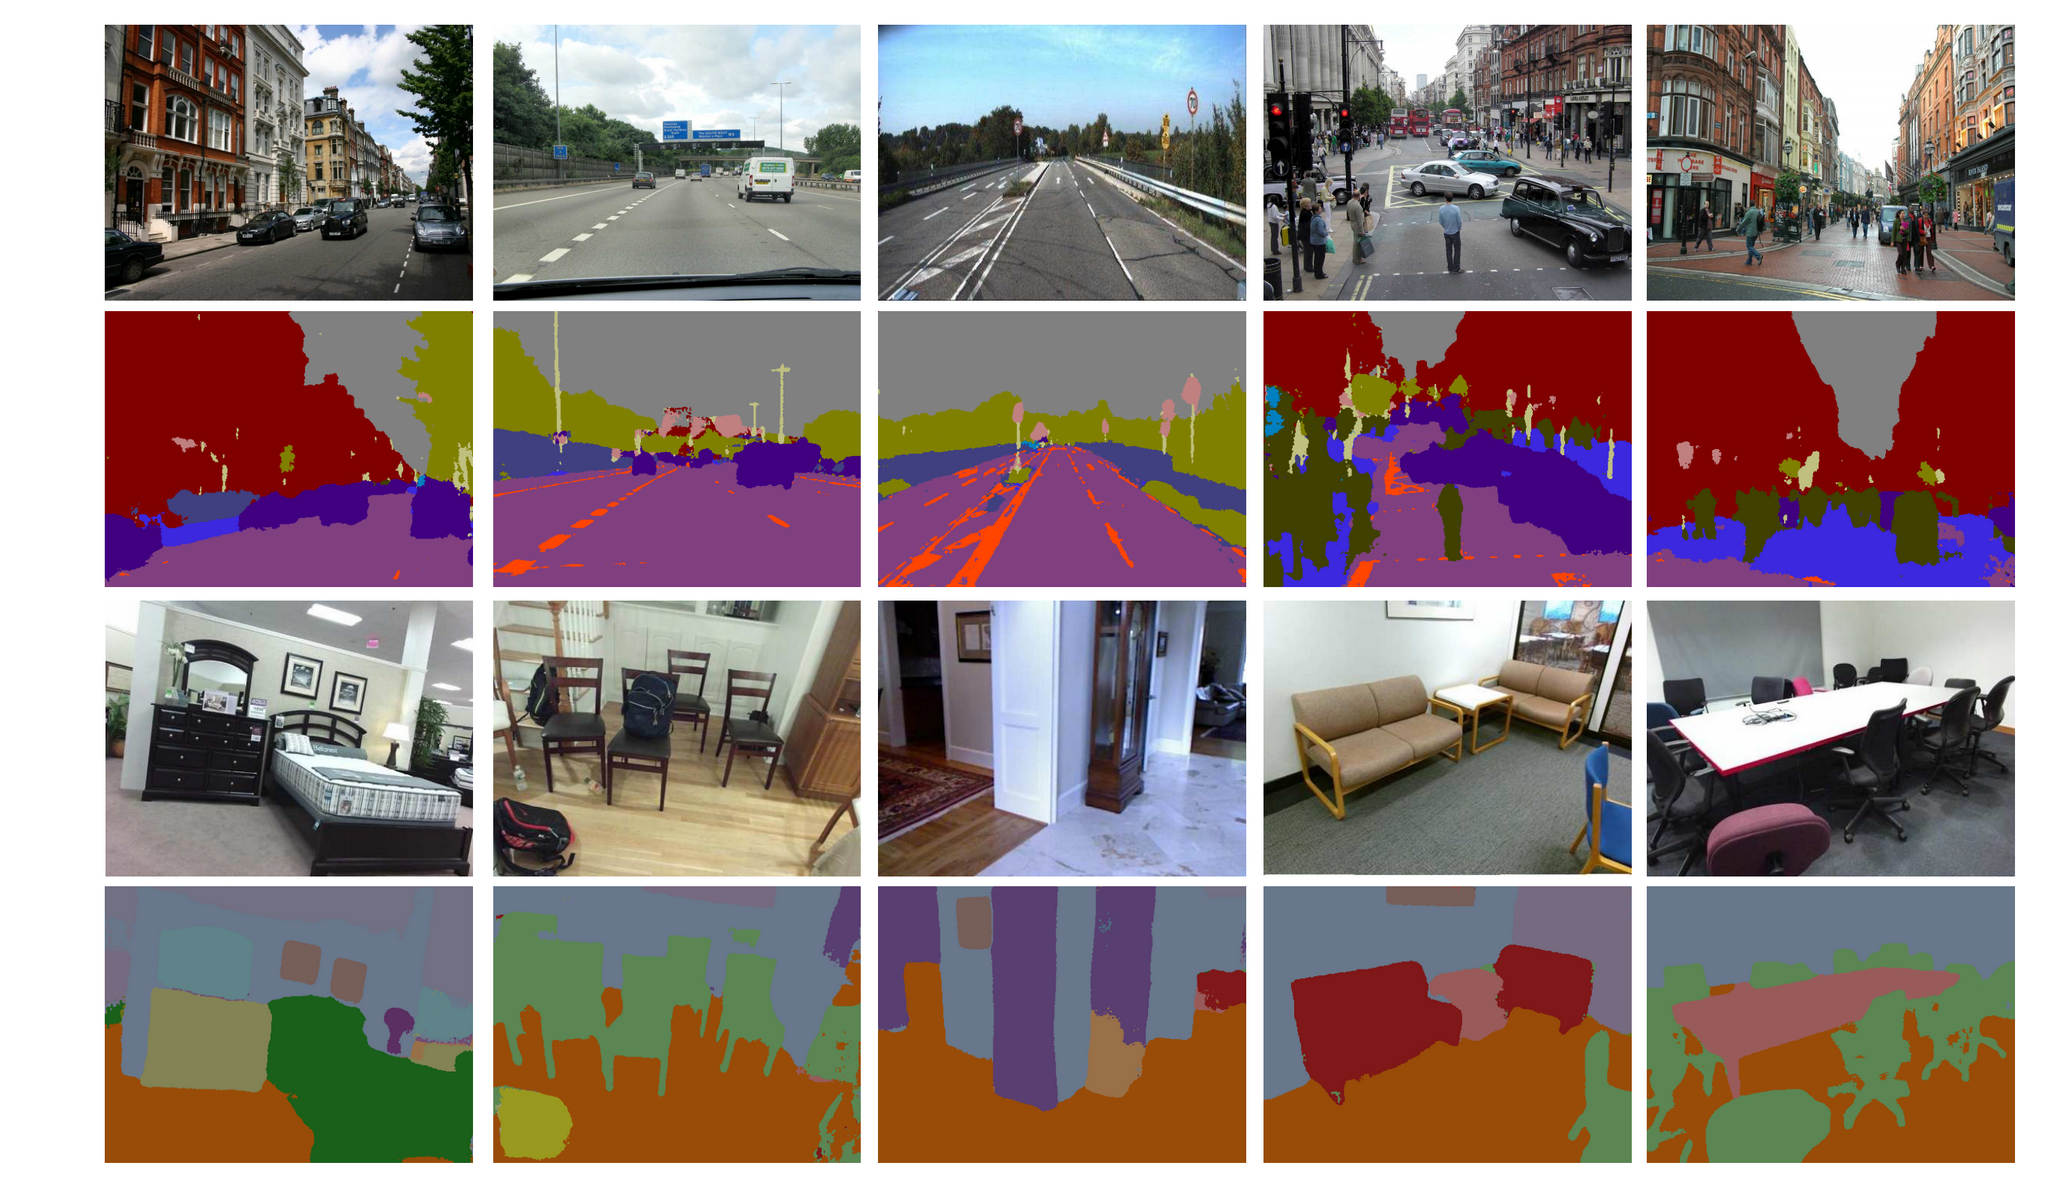
\includegraphics[width=0.65\linewidth]{images/scr1.png}
  \captionof{figure}{Segnet predictions on road scene and indoor scenes}
\end{minipage}  
  
